\ifdefined\included
\else
\documentclass[english,a4paper,11pt,twoside]{StyleThese}
\usepackage{amsmath,amssymb}             % AMS Math
\usepackage[T1]{fontenc}
\usepackage[utf8x]{inputenc}
\usepackage{babel}
\usepackage{datetime}

\usepackage{lmodern}
\usepackage{tabularx}
%\usepackage{tabular}
\usepackage{multirow}

\usepackage{subfigure}
\usepackage{fancyvrb}
\usepackage{algorithmic}
\usepackage{algorithm}
\usepackage{mathtools}


\usepackage{hhline}
\usepackage[left=1.5in,right=1.3in,top=1.1in,bottom=1.1in,includefoot,includehead,headheight=13.6pt]{geometry}
\renewcommand{\baselinestretch}{1.05}

% Table of contents for each chapter

\usepackage[nottoc, notlof, notlot]{tocbibind}
\usepackage{minitoc}
\setcounter{minitocdepth}{2}
\mtcindent=15pt
% Use \minitoc where to put a table of contents

\usepackage{aecompl}


% Glossary / list of abbreviations

\usepackage[intoc]{nomencl}
\iftoggle{ThesisInEnglish}{%
\renewcommand{\nomname}{Glossary}
}{ %
\renewcommand{\nomname}{Liste des Abréviations}
}

\newcommand{\accom}[1]{\textcolor{red}{[#1]}}

\makenomenclature

% My pdf code

\usepackage{ifpdf}

\ifpdf
  \usepackage[pdftex]{graphicx}
  \DeclareGraphicsExtensions{.jpg}
  \usepackage[a4paper,pagebackref,hyperindex=true]{hyperref}
  \usepackage{tikz}
  \usetikzlibrary{arrows,shapes,calc}
\else
  \usepackage{graphicx}
  \DeclareGraphicsExtensions{.ps,.eps}
  \usepackage[a4paper,dvipdfm,pagebackref,hyperindex=true]{hyperref}
\fi

\graphicspath{{.}{images/}}

%% nicer backref links. NOTE: The flag ThesisInEnglish is used to define the
% language in the back references. Read more about it in These.tex

\iftoggle{ThesisInEnglish}{%
\renewcommand*{\backref}[1]{}
\renewcommand*{\backrefalt}[4]{%
\ifcase #1 %
(Not cited.)%
\or
(Cited in page~#2.)%
\else
(Cited in pages~#2.)%
\fi}
\renewcommand*{\backrefsep}{, }
\renewcommand*{\backreftwosep}{ and~}
\renewcommand*{\backreflastsep}{ and~}
}{%
\renewcommand*{\backref}[1]{}
\renewcommand*{\backrefalt}[4]{%
\ifcase #1 %
(Non cité.)%
\or
(Cité en page~#2.)%
\else
(Cité en pages~#2.)%
\fi}
\renewcommand*{\backrefsep}{, }
\renewcommand*{\backreftwosep}{ et~}
\renewcommand*{\backreflastsep}{ et~}
}

% Links in pdf
\usepackage{color}
\definecolor{linkcol}{rgb}{0,0,0.4} 
\definecolor{citecol}{rgb}{0.5,0,0} 
\definecolor{linkcol}{rgb}{0,0,0} 
\definecolor{citecol}{rgb}{0,0,0}
% Change this to change the informations included in the pdf file

\hypersetup
{
bookmarksopen=true,
pdftitle="Joint Action for Human-Robot Interaction",
pdfauthor="Sandra DEVIN", %auteur du document
pdfsubject="Thesis", %sujet du document
%pdftoolbar=false, %barre d'outils non visible
pdfmenubar=true, %barre de menu visible
pdfhighlight=/O, %effet d'un clic sur un lien hypertexte
colorlinks=true, %couleurs sur les liens hypertextes
pdfpagemode=None, %aucun mode de page
pdfpagelayout=SinglePage, %ouverture en simple page
pdffitwindow=true, %pages ouvertes entierement dans toute la fenetre
linkcolor=linkcol, %couleur des liens hypertextes internes
citecolor=citecol, %couleur des liens pour les citations
urlcolor=linkcol %couleur des liens pour les url
}

% definitions.
% -------------------

\setcounter{secnumdepth}{3}
\setcounter{tocdepth}{2}

% Some useful commands and shortcut for maths:  partial derivative and stuff

\newcommand{\pd}[2]{\frac{\partial #1}{\partial #2}}
\def\abs{\operatorname{abs}}
\def\argmax{\operatornamewithlimits{arg\,max}}
\def\argmin{\operatornamewithlimits{arg\,min}}
\def\diag{\operatorname{Diag}}
\newcommand{\eqRef}[1]{(\ref{#1})}

\usepackage{rotating}                    % Sideways of figures & tables
%\usepackage{bibunits}
%\usepackage[sectionbib]{chapterbib}          % Cross-reference package (Natural BiB)
%\usepackage{natbib}                  % Put References at the end of each chapter
                                         % Do not put 'sectionbib' option here.
                                         % Sectionbib option in 'natbib' will do.
\usepackage{fancyhdr}                    % Fancy Header and Footer

% \usepackage{txfonts}                     % Public Times New Roman text & math font
  
%%% Fancy Header %%%%%%%%%%%%%%%%%%%%%%%%%%%%%%%%%%%%%%%%%%%%%%%%%%%%%%%%%%%%%%%%%%
% Fancy Header Style Options

\pagestyle{fancy}                       % Sets fancy header and footer
\fancyfoot{}                            % Delete current footer settings

%\renewcommand{\chaptermark}[1]{         % Lower Case Chapter marker style
%  \markboth{\chaptername\ \thechapter.\ #1}}{}} %

%\renewcommand{\sectionmark}[1]{         % Lower case Section marker style
%  \markright{\thesection.\ #1}}         %

\fancyhead[LE,RO]{\bfseries\thepage}    % Page number (boldface) in left on even
% pages and right on odd pages
\fancyhead[RE]{\bfseries\nouppercase{\leftmark}}      % Chapter in the right on even pages
\fancyhead[LO]{\bfseries\nouppercase{\rightmark}}     % Section in the left on odd pages

\let\headruleORIG\headrule
\renewcommand{\headrule}{\color{black} \headruleORIG}
\renewcommand{\headrulewidth}{1.0pt}
\usepackage{colortbl}
\arrayrulecolor{black}

\fancypagestyle{plain}{
  \fancyhead{}
  \fancyfoot{}
  \renewcommand{\headrulewidth}{0pt}
}

%\usepackage{MyAlgorithm}
%\usepackage[noend]{MyAlgorithmic}
\usepackage[ED=MITT - STICIA, Ets=INP]{tlsflyleaf}
%%% Clear Header %%%%%%%%%%%%%%%%%%%%%%%%%%%%%%%%%%%%%%%%%%%%%%%%%%%%%%%%%%%%%%%%%%
% Clear Header Style on the Last Empty Odd pages
\makeatletter

\def\cleardoublepage{\clearpage\if@twoside \ifodd\c@page\else%
  \hbox{}%
  \thispagestyle{empty}%              % Empty header styles
  \newpage%
  \if@twocolumn\hbox{}\newpage\fi\fi\fi}

\makeatother
 
%%%%%%%%%%%%%%%%%%%%%%%%%%%%%%%%%%%%%%%%%%%%%%%%%%%%%%%%%%%%%%%%%%%%%%%%%%%%%%% 
% Prints your review date and 'Draft Version' (From Josullvn, CS, CMU)
\newcommand{\reviewtimetoday}[2]{\special{!userdict begin
    /bop-hook{gsave 20 710 translate 45 rotate 0.8 setgray
      /Times-Roman findfont 12 scalefont setfont 0 0   moveto (#1) show
      0 -12 moveto (#2) show grestore}def end}}
% You can turn on or off this option.
% \reviewtimetoday{\today}{Draft Version}
%%%%%%%%%%%%%%%%%%%%%%%%%%%%%%%%%%%%%%%%%%%%%%%%%%%%%%%%%%%%%%%%%%%%%%%%%%%%%%% 

\newenvironment{maxime}[1]
{
\vspace*{0cm}
\hfill
\begin{minipage}{0.5\textwidth}%
%\rule[0.5ex]{\textwidth}{0.1mm}\\%
\hrulefill $\:$ {\bf #1}\\
%\vspace*{-0.25cm}
\it 
}%
{%

\hrulefill
\vspace*{0.5cm}%
\end{minipage}
}

\let\minitocORIG\minitoc
\renewcommand{\minitoc}{\minitocORIG \vspace{1.5em}}

\usepackage{multirow}
%\usepackage{slashbox}

\newenvironment{bulletList}%
{ \begin{list}%
	{$\bullet$}%
	{\setlength{\labelwidth}{25pt}%
	 \setlength{\leftmargin}{30pt}%
	 \setlength{\itemsep}{\parsep}}}%
{ \end{list} }

\newtheorem{definition}{Définition}
\renewcommand{\epsilon}{\varepsilon}

% centered page environment

\newenvironment{vcenterpage}
{\newpage\vspace*{\fill}\thispagestyle{empty}\renewcommand{\headrulewidth}{0pt}}
{\vspace*{\fill}}

\usepackage{tablefootnote}

\sloppy
\begin{document}
\setcounter{chapter}{2} %% Numéro du chapitre précédent ;)
\dominitoc
\faketableofcontents
\fi

\chapter{Taking Humans Mental States into account while executing Shared Plans}
\minitoc

\label{ch:MS}

\section{Motivations}

When collaborating with humans, it is primordial for the robot to not consider humans as obstacles or tools impacting the environment. As humans are social creatures, the robot must take into account their comfort and so, their point of view. Several works already allow robots to estimate humans perspective and beliefs concerning its environment. In order to improve human-robot Joint Action, the robot must be able to take these information into account when taking decision on how to act or what to communicate. Even if several works have been done on how to integrate humans perspective in dialogue or use it to help the understanding of humans behavior, there is still a gap when it came to use it during Shared Plan execution. This work aims to start filling this gap by extending the robot knowledge on humans mental states to the joint task and using it to better communicate during Shared Plan execution. It has been the subject of a publication into the HRI conference \cite{devin2016implemented}.

\section{Theory of Mind}

\subsection{Social Sciences literature}

Theory of the Mind (ToM) refers to the ability humans have to recognize and attribute mental states not only to themselves but to other people, to understand that feelings and beliefs we have may be different than others and to take others mental states into account when taking decisions. ToM has been deeply studied in psychology, notably in the developmental domain \cite{baron1985does, premack1978does}. \cite{verbrugge2008learning} defines what is called "order" of ToM:
\begin{quote}
"To have a first-order ToM is to assume that someone’s beliefs,
thoughts and desires influence one’s behavior. A first-order thought could be: ‘He does not know that his book is on the table’. In second-order ToM it is also recognized that to predict others’ behavior, the desires and beliefs that they have of one’s self and the predictions of oneself by others must be taken into account. So, for example, you can realize that what someone expects you to do will affect his behavior. For example, ‘(I know) he does not know that I know his book is on the table’ would be part of my second-order ToM. To have a third-order ToM is to assume others to have a second-order ToM, etc."
\end{quote}
There is an infinitesimal numbers of orders, however, studies shown that orders above the second one do not help in cooperative tasks \cite{de2014theory} and above the third one do not help for competitive games \cite{de2014theory}.


\begin{figure*}[!h]
    \centering
    \subfigure[Perceptual perspective taking: two individuals can have a different representation of their environment considering their locations.]{
        \centering
        \includegraphics[width=0.4\textwidth]{figs/Chapter3/perceptual.jpg}
       \label{subfig:perceptual}
   }
    %~
    \subfigure[Conceptual perspective taking: here Bob attributes to Alice a belief concerning the box. He thinks Alice thinks the box is empty.]{
        \centering
        \includegraphics[width=0.4\textwidth]{figs/Chapter3/conceptual.jpg}
       \label{subfig:conceptual}
    }
    \caption{Illustration of perceptual and conceptual perspective taking.}
\end{figure*}

ToM includes the notion of perspective taking: the capacity for a person to reason by taking the point of view of someone else. Studied in literature \cite{tversky1999speakers, flavell1992perspectives}, perspective taking is crucial during humans interaction and studies have demonstrate that individuals who lack of this ability have difficulties in their daily social interactions \cite{frick2014picturing}. Two levels of perspective taking are defined in \cite{flavell1977development}: perceptual and conceptual perspective taking. Perceptual perspective taking design the capacity of a person to understand that others have a different perception of the world (fig~\ref{subfig:perceptual}). Conceptual perspective taking designs the capacity of a person to attribute beliefs and feelings to others (fig~\ref{subfig:conceptual}).

\begin{figure}[!h]
	\centering
    \includegraphics[width=0.7\textwidth]{figs/Chapter3/sally.jpg}
    \caption{The Sally and Anne test: it allows to check the capacity of someone to attribute a false-belief to another person. Illustration from the work of Axel Scheffler.}
    \label{fig:sally}
\end{figure}

To check if an individual has ToM capacities, several tests have been developed in psychology. One of the most famous is the Sally and Anne test (fin~\ref{fig:sally}). This test allows to check the capacity of someone to attribute a false-belief to another person and have been reused in robotics to validate robots perspective taking abilities.

\subsection{Robotics background}

One of the pioneer work in robotics Theory of Mind is \cite{scassellati2002theory}. Scassellati presents two models from social sciences (Leslie \cite{leslie1984spatiotemporal} et Baron-Cohen \cite{baron1997mindblindness}) and proposes a model on how to implement ToM in robotics. However, the implementation of this model did not go further than perception level.

Then, several works have been done in order to endow robots with perspective taking abilities. Using ACT-R architecture \cite{anderson2004integrated}, the team of Hiatt and Trafton models mechanisms used during the Sally and Anne test and constructs a model that learns to deal with false belief in order to pass this test \cite{hiatt2010cognitive}. They extend this work to second-order in \cite{hiatt2015understanding} and to spatial reasoning in \cite{hiatt2004cognitive}. The Sally and Anne test has also been passed in \cite{milliez2014framework} where the robot constructs a semantic representation of the world from its partners point of view. In \cite{berlin2006perspective}, authors present a way to record different beliefs of other agents and so to have a memory of perspective taking. Finally, \cite{johnson2005perspective} presents a system which computes perspective taking based on forward and inverse visual models.

Perspective taking abilities have been used in robotics for several purposes. It has been used in \cite{hiatt2011accommodating} to deal with uncertainty in humans behavior and in \cite{ros2010solving} to solve ambiguous references to an object. One important application of perspective taking is action recognition. \cite{johnson2005perceptual} takes the visual point of view of humans to improve action recognition, Dynamic Bayesian Networks (DBN) are used in \cite{baker2014modeling} or inverse reinforcement learning  in \cite{nagai2015probabilistic}. The human perspective is also used in \cite{breazeal2006using} to learn a task from a situation that can be ambiguous from the robot point of view and in \cite{gray2014manipulating} to choose actions with the adequate effects in order to manipulate humans mental models. Finally, \cite{gorur2017toward} uses perspective taking to infer humans intention and adapt robot decision.

Concerning Shared Plans, perspective taking can be used to help their elaboration in order to add communication actions to solve divergent beliefs \cite{guitton2012belief}. Then, the human perspective is used to share the plan with a level of details depending of human knowledge \cite{milliez2016using}. However, there is no works for now concerning the management of Shared Plans execution taking into account the human point of view. 

\section{Assumptions}


The work presented in this chapter concerns the estimation of humans knowledge on the task and its use to help the Shared Plan execution. To do so, we make several assumptions:

\paragraph{Commitment:} we do not focus in this works on issues related to commitment. Consequently, we consider here that the joint goal has already been established. We also consider that none of the humans will abort the goal unless he knows that the goal is not achievable any more.

\paragraph{Shared Plan:} the focus of this work concerns rather the Shared Plan execution than the Shared Plan elaboration. In the examples presented in Sec.~\ref{sec:resultsTOM}, the Shared Plan is computed by the robot, however, the processes presented in this chapter hold regardless of the way the robot gets the Shared Plan (e.g. it can be imposed by a human or negotiated through dialogue). This chapter will treat only the issues related to ToM usage in Shared Plan execution, the rest of Shared Plan management will be more developed in Chapter \ref{ch:SP}.

\paragraph{ToM order:} this work implements a first-order ToM for the robot (i.e. the robot has knowledge about the human knowledge on the task), the higher orders are not managed for now.

\paragraph{Humans perception:} we make the assumption here that a human will see and understand an action of another agent (mainly robot actions) when he is present and looking at the agent. We
also assume that when he is present, the human is able to hear and understand the information verbalized by the robot.

\paragraph{Robot capacities:} we consider that the robot is able to perform simple high level actions like Pick, Place or Drop. We also assume that the robot is able to ask to a human to perform an action and to inform him about the state of the environment, the goal or an action. The robot is able to detect and localize objects and agents
and to recognize simple high level actions performed by a human like Pick, Place or Drop. Let us also note that the ways the robot achieves actions (e.g. human-aware motion planning and execution) and recognizes humans’ actions are outside of the scope of this chapter.

\paragraph{Communication:} this work consists mainly in finding which information to give to the human and at which time. We do not focus here on the how we give these information (here we use the basic dialogue module described in Chapter~\ref{ch:Sup} but more complex communication mechanisms can be envisioned). 

\section{Estimating Humans Mental States}

As stated previously, the goal of this work is to fill the gap between existing perspective taking abilities of the robot and Shared Plan execution. A first step to do so is to extend the knowledge of the robot concerning humans mental states to information concerning the Shared Plan. As saw in Chapter~\ref{ch:Sup}, the mental state of a human H will be described as:
$$MS(H) = <g_H, g_R(H), SP(H), WS(H)>$$
where $g_H$ is the goal the robot estimates the human is engaged in, $g_R(H)$ is the goal the robot estimates the human thinks the robot is performing, and $SP(H)$ and $WS(H)$ are the estimation of the Shared Plan and the World State from the human point of view. 

The process to estimate the humans mental states will be noted in the following of the thesis as the operator:
$$MS(H) \leftarrow ESTIMATE\_MS(MS(H), TS)$$

with $TS$ the state of the task from the robot point of view as stated in Chapter~\ref{ch:Sup}.
We will see now how we estimates each of the mental states components.

\subsection{Goal management ($g_H$ and $g_R(H)$ computation)}

As stated previously, the focus of this work is not put on the goal management. Consequently, the computation of humans mental states concerning goals remains basic. However, a more complex one can be envisioned, for example using intention recognition, with the same representation. As a reminder, a goal is defined as:
$$g = <Name_g, Actors_g, Params_g, Obj_g>$$

As we consider humans automatically engaged in the goal, as soon as the robot starts executing a goal, all actors of the goal are considered to have the same goal:
$$ \forall H \in Actors_{g_R}, \ g_H = g_R$$
We also make the basic assumption that all humans who see the robot are aware of its goal:
$$ \forall H  \ | <Robot, isVisibleBy, H> \in WS, \ g_R(H) = g_R$$
For a goal to be considered achieved by an agent (it holds for human mental states as well as the robot mental state), this agent needs to have all the objectives of the goal in its knowledge (it means that accordingly to its knowledge, the desired world state has been reached):
$$ \forall H, \ \forall g  \ | \ Obj_g \in WS(H), \ label_g = DONE$$
The robot will consider a goal failed if it does not find a plan any more to achieve it. Concerning the humans, they can be informed through dialogue by the robot of the failure (or success) of a goal.

\subsection{Shared Plan management ($SP(H)$ computation)}

As a reminder, the representation of the Shared Plan $SP$ from a human H point of view is represented as:
$$SP(H) = <id_p(H), A_p(H), L_p(H)>$$
where $id_p(H)$ is used to identify the plan, $A_p(H)$ are the actions composing the plan and $L_p(H)$ the links representing the order the actions should be executed (causal links).

As we consider in this thesis Shared Plans with action allocation evolving during the execution, we made the choice not to share the plan and communicate about actions only when it is not implicit (more details in Chapter~\ref{ch:SP}). Hence, we consider that the Shared Plan of the human is always the same as the robot one, only the state of the actions composing the plan will change:
$$SP(H) = <id_p, A_p(H), L_p>$$

A link $l \in L_p$ can be describe as:
 $$l = \langle prev_l, \ next_l \rangle$$
where $prev_l$ is the id of the action which needs to be achieved before the action with the id $next_l$ is performed. 

The actions composing the plan $A_p(H)$ can be decomposed as:
$$A_p(H) = <A_{prev}(H), A_{cur}(H), A_{next}(H), A_{later}(H)>$$
where $A_{prev(H)}$ are the actions of the plan the human thinks already executed, $A_{cur}(H)$ the actions the human thinks currently executed, $A_{next}(H)$ the actions the human thinks which can be performed and $A_{later}(H)$ the actions the human thinks to be executed in the future. Each action $a$ in $A_{prev}(H)$ is associated with a label noted $label_a$ which can be equal either to DONE, FAILED or ABORTED.

By default, when a Shared Plan is computed by the robot, all actions are put in $A_{later}(H)$. When the robot performs an action or detects an action execution from a human, it considers the human is aware of the action if he can see the actors of the action:

\begin{center}
$a \in A_{cur} \ \& \ (<Ag_a, isVisibleBy, Human> \in WS \ \| \ Human \in Ag_a)$ 

$\Rightarrow a \in A_{cur}(H)$
\end{center}

In a same way, at the end of the execution, the action goes in $A_{prev}(H)$ with the label corresponding to the success or the failure of the action if the human performs or saw the actors of the actions at the end of the action.

We also consider that a human can infer that an action has been done if it knows that the action was in progress or on its way to be done and it can see the effects of the action:

\begin{center}
$(a \in A_{cur}(H) \ \| \ a \in A_{next}(H)) \ \& \ Effects_{a} \in WS(H)$ 

$\Rightarrow a \in A_{prev}(H) \ \& \ label_a(H) = DONE$
\end{center}

In a same way, we consider that if a human knows that an action was in progress and can see the actors of the action while there are not performing the action any more, he considers the action DONE:

\begin{center}
$a \in A_{next}(H) \ \& \ a \in A_{prev} \ \& \ <Ag_a, isVisibleBy, Human> \in WS$

$\Rightarrow a \in A_{prev}(H) \ \& \ label_a(H) = DONE$
\end{center}

Finally, the actions are set in $A_{next}(H)$ considering causal links and preconditions:

\begin{center}
$a \in A_{next}(H) \Leftrightarrow Precs_{a} \in WS(H) \ \& \ (\forall l \in L_p$ 

$| \ next_l = id_a, \exists \ ap \in A_{prev}(H) \ | \ (id_{ap} = prev_l \ \& \ label_{ap}(H)  = DONE))$
\end{center}

The robot can also inform a human about the state of an action, in which case the given information will be add to the human mental state.

\subsection{World State management ($WS(H)$ computation)}
\label{subsec:worldstate}

We saw that the perspective taking abilities of the robot allow it to estimate the human perception of his environment \cite{milliez2014framework}. However, this previous work only concerns information about the environment which are perceivable. Indeed, for this work we will consider two kinds of predicates to describe the state of the environment:
\begin{itemize}
\item \textbf{Observable predicates:} they concern what the agent can observe about the world state. These predicates mainly represent the affordances of all agents (e.g. isVisibleBy, isReachableBy) and the relations between objects (e.g. isOn, isIn) visible to them. They are computed continuously by the Situation Assessment module (TOASTER) from the robot and humans point of views based on geometric computations and perspective taking algorithms.
\item \textbf{Non-observable predicates:} they concern information that the agent can not observe (e.g. the fact that an opaque bottle is empty). These predicates are not managed by TOASTER which reason on what is visible by the agents. We consider two ways for an agent to be aware of a non-observable predicate. First, it can perform or see an action which has this predicate in its side effects:
$$\forall a \ \in \ A_{prev} \ | \ label_{a} \ = \ DONE \Rightarrow Effects_{a} \rightarrow WS$$
(likewise with $A_{prev}(H)$ and $WS(H)$). A human can also be aware of a non-observable predicate if he is informed of it by the robot.
\end{itemize}


\section{Mental States for Shared Plans execution}

We saw in the previous section how we estimate humans mental states concerning the shared task. We will see now how we use them to communicate during the Shared Plan execution. Indeed, when two humans share a plan, they usually do not communicate all along the plan execution. Only the \textit{meshing subplans} of the plan need to be shared \cite{bratman1993shared}. Consequently, the robot should inform humans about elements of the shared plan only when it considers that the divergent belief might have an impact on the joint activity in order to not be intrusive by giving them information which they do not need or which they can observe or infer by themselves. The process of monitoring the divergent beliefs and solving them if needed which will be described in this section will be noted in the following of the thesis as:
$$SOLVE\_DB(MS(H), TS)$$

\subsection{Weak achievement goal}

If we follow the definition of \textit{weak achievement goal} in \cite{cohen1991teamwork}, if the robot knows that the current goal has been achieved or is not possible anymore, it has to inform its partners. Accordingly, we consider that, when, in the robot knowledge, the label of a goal is DONE (resp. ABORTED) and the robot estimates that a human does not consider it DONE (resp. ABORTED), the robot informs him about the achievement (resp. abandoning) of the goal (if the agent is not here or is busy with something else, the robot will do it as soon as the agent is available).

\begin{algorithm}
\caption{Weak achievement goal}
\label{alg:informGoal}
\begin{algorithmic}
\IF {$\exists \ g \ | \ (label_g = DONE \ \& \ label_g(H) \neq DONE) \ \| \ (label_g = ABORTED \ \& \ label_g(H) \neq ABORTED)$ \hfill \textit{$\vartriangleright$ There is a divergent belief to solve}
\STATE}
\STATE Inform($g$)\hfill \textit{$\vartriangleright$ The robot informs the human about the state of the goal}
\ENDIF
\end{algorithmic}
\end{algorithm} 

\subsection{Before humans action}

A divergent belief of a human partner can be an issue when it is related to an action that he has to perform. To avoid that a human misses information to execute his part of the Shared Plan, each time the robot estimates that a human has to perform an action (action in $A^H_{next}$) it checks if the human is aware that he has to and can perform the action (the action should also be in $A^H_{next}(H)$).
In order not to give too much information at the same time, and as not yet allocated actions can also be performed by the robot, the robot checks for actions in $A^X_{next}(H)$ only if the human does not have any other actions to perform. If there is a divergent belief, there are two possible reasons:
\begin{itemize}
\item The human misses information about previous achieved actions to know that his action has to be performed now according to the plan. The robot checks the label of all actions linked to the first one with the plan links and informs about the achievement of all actions with a label different of DONE in the estimation of the human knowledge.
\item The human misses information about the world state to know that his action is possible. In such case, the robot looks into the preconditions of the actions and informs the human about all those the human is not aware of.
\end{itemize}
The given algorithm to solve this kind of divergent belief is summarized in Alg.~\ref{alg:checkHumanAction}.


\begin{algorithm}
\caption{Checking humans actions}
\label{alg:checkHumanAction}
\begin{algorithmic}
\IF {$(\exists \ action \in A^H_{next} \ | \ action \notin A^H_{next}(H)) \ \| \ (A^H_{next} = \emptyset \ \& \ \exists \ action \in A^X_{next} \ | \ action \notin A^X_{next}(H))$}
\STATE \hfill \textit{$\vartriangleright$ There is a divergent belief to solve}
\IF {$\exists \ a \in A_{p} \ | \ (\exists \ l \in L_p \ | \ next_l = action \ \& \ prev_l = a) \ \& \ (a \notin A_{prev}(H) \ \| \ label_a(H) \neq DONE))$}
\STATE Inform($a$)\hfill \textit{$\vartriangleright$ The robot says to the human that the action is done}
\ENDIF
\IF {$\exists p \in Precs_{action} \ | \ p \notin WS(H))$}
\STATE Inform($p$)\hfill \textit{$\vartriangleright$ The robot informs about the missing precondition}
\ENDIF
\ENDIF
\end{algorithmic}
\end{algorithm} 

\subsection{Preventing mistakes}

A divergent belief of a human partner can also be an issue if it leads him to perform an action that should not be perform now according to the plan. To prevent this, for each action that the robot estimates the human thinks he has to execute (action in $A^H_{next}(H)$), the robot checks if the action really needs to be performed (the action should also be in $A^H_{next}$). In the same way, the robot also checks the actions not yet allocated as the human can perform them (action in $A^X_{next}(H)$ which is not in $A^X_{next}$). If there is a divergent belief, the robot corrects the human divergent belief by two different ways:
\begin{itemize}
\item The human can think that a previous action has been achieved successfully while it is not the case leading him to think he has to perform another action. The robot looks in all actions linked to the first one by the plan links and informs about their state if it is different in the estimation of the human knowledge and in the robot knowledge.
\item The human can have a divergent belief concerning the world state that leads him to think that his action is possible while it is not the case. The robot looks into the preconditions of the action and informs about divergent beliefs.
\end{itemize}
The given algorithm to solve this kind of divergent belief is summarized in Alg.~\ref{alg:checkMistakes}.


\begin{algorithm}
\caption{Preventing mistakes}
\label{alg:checkMistakes}
\begin{algorithmic}
\IF {$\exists \ action \in {A^H_{next}(H) \ \cup \ A^X_{next}(H)} \ | \ action \notin \{A^H_{next} \ \cup \ A^X_{next}\}$}
\STATE \hfill \textit{$\vartriangleright$ There is a divergent belief to solve}
\IF {$\exists \ a \in A_{p} \ | \ (\exists \ l \in L_p \ | \ next_l = action \ \& \ prev_l = a) \ \& \ (label_a(H) = DONE) \ \& \ (a \notin A_{prev} \ \| \ label_a \neq DONE))$}
\STATE Inform($a$)\hfill \textit{$\vartriangleright$ The robot informs about the state of the action}
\ENDIF
\IF {$\exists p \in Precs_{action} \ | \ p \in WS(H) \ \& \ p \notin WS)$}
\STATE Inform($p$)\hfill \textit{$\vartriangleright$ The robot informs about the wrong precondition}
\ENDIF
\ENDIF
\end{algorithmic}
\end{algorithm} 


\subsection{Signal robot actions}

When the robot is about to perform an action, it checks if it estimates that the humans are aware that it will act (the action should also in $A^R_{next}(H)$). If it is not the case, the robot signals its action before performing it (Alg.~\ref{alg:signalActions}).

\begin{algorithm}
\caption{Signal robot actions}
\label{alg:signalActions}
\begin{algorithmic}
\IF {$\exists \ action \in A^R_{next} \ | \ action \notin A^R_{next}(H)$ \hfill \textit{$\vartriangleright$ There is a divergent belief to solve}
\STATE}
\STATE Signal($action$)\hfill \textit{$\vartriangleright$ The robot signals its action}
\ENDIF
\end{algorithmic}
\end{algorithm} 


\subsection{Inaction and uncertainty}

Even if the robot estimates that the human is aware that he has to act (there is action(s) in $A^H_{next}(H)$), it is possible that the human still does not perform his action(s). If the human is already busy by something else (there is an action in $A^H_{cur}$) or if it is not currently engaged in the task, the robot waits for the human to be available. If the human is not considered busy by the robot, the robot first considers that its estimation of the human mental state can be wrong, and that, in reality, the human is not aware that he should act. Consequently, the robot asks the human specifically to perform the action. If the human still does not act while the action has been asked, the robot considers the action failed, aborts the current plan and tries to find an alternative plan excluding that action.


\section{Results}

\label{sec:resultsTOM}

\subsection{Tasks}

In order to evaluate the benefits of our method during human-robot interaction, we will use two different tasks. We will first show an illustrative example of one possible scenario of the first task, and then, we will run simulations on these two tasks in order to get objective measurement of the performance of the system in simulation. The system will be evaluated in a real situation latter in Chapter~\ref{ch:Eval}.

\paragraph{"Clean the table" scenario}

In this example, a PR2 robot and a human have to clean a table together. To do so, they need to remove all items from this table, sweep it, and re-place all previous items. The initial world state is the one in Fig.~\ref{fig:initClean}. We consider that the grey book is reachable only by the robot, the blue book only by the human and the white book by both agents. The human and the robot have the ability to pick objects and place them into another support. Only the robot has the capacity to sweep the table. The initial plan produced to achieve the goal is shown in Fig.~\ref{fig:initPlanClean}.

\begin{figure}[!h]
	\centering
    \includegraphics[width=0.6\textwidth]{figs/Chapter3/cleanWithNames.png}
    \caption{Initial situation of the "Clean the table" scenario.}
    \label{fig:initClean}
\end{figure}

\paragraph{"Inventory" scenario}

In this example, a human and a PR2 robot have to make an inventory together. At the beginning of the task, both agents have coloured objects near them as well as a coloured box (initial world state in Fig.~\ref{fig:initInventory}). These coloured objects need to be scanned and then, stored in the box of the same colour. To do so, both agents can pick objects and place them in the table in a way reachable by the other agent. They also both have the ability to drop objects in the box near them. Finally, only the robot can scan an object, it consists of orienting its head and turning on a red light in the direction of a reachable object. 

\begin{figure}[!h]
	\centering
    \includegraphics[width=0.6\textwidth]{figs/Chapter3/initInventory.png}
    \caption{Initial situation of the "Inventory" scenario.}
    \label{fig:initInventory}
\end{figure}



\subsection{Illustrating scenario}

We will first illustrate the benefits of the work presented in this chapter with an example. This example is based on the "Clean the table" task presented previously. At the beginning of the interaction the robot computes the plan Fig.~\ref{fig:initPlanClean}. 

\begin{figure}[!h]
	\centering
    \includegraphics[width=0.7\textwidth]{figs/Chapter3/InitCleanPlan.png}
    \caption{Initial plan of the "Clean the table" scenario. }
    \label{fig:initPlanClean}
\end{figure}


The robot starts to pick and place the grey book on the light-coloured shelf. The human picks and places the blue book on the dark-coloured shelf then leaves (Fig.~\ref{subfig:humanLeave}).

\begin{table}[!h]
\begin{center}
\begin{tabular}{|c|c|c|c||c|c|c|c|}
\hline
\multicolumn{4}{|c||}{Robot} & \multicolumn{4}{c|}{Human}\\
\hline
$A_{prev}$ & $A_{cur}$ & $A_{next}$ & $A_{ready}$ & $A_{prev}$ & $A_{cur}$ & $A_{next}$ & $A_{ready}$\\
\hline
\hline
1 & 0 & 2 & 3, 4, 5, 6 & 1 & 0 & 2 & 3, 4, 5, 6\\
\hline
\end{tabular}
\end{center}
\caption{Knowledge of the robot and estimation of the human knowledge after the human left. The numbers represent the actions id as stated in the plan Fig.~\ref{fig:initPlanClean}.}
\label{table:results}
\end{table}

The robot ends its action. At this point, the only possible action of the plan has to be done by the human. The robot waits a few time for the human and then, as the human does not come back (and so does not execute its action), aborts the current plan and computes a new one where it removes the last book (Fig.~\ref{fig:newplan}).
The robot picks and places the white book on the light-coloured shelf and sweeps the table (Fig.~\ref{subfig:robotSweep}).

\begin{figure}[!h]
	\centering
    \includegraphics[width=0.7\textwidth]{figs/Chapter3/SecondCleanPlan.png}
    \caption{Second plan of the "Clean the table" scenario.}
    \label{fig:newplan}
\end{figure}

\begin{table}[!h]
\begin{center}
\begin{tabular}{|c|c|c|c||c|c|c|c|}
\hline
\multicolumn{4}{|c||}{Robot} & \multicolumn{4}{c|}{Human}\\
\hline
$A_{prev}$ & $A_{cur}$ & $A_{next}$ & $A_{ready}$ & $A_{prev}$ & $A_{cur}$ & $A_{next}$ & $A_{ready}$\\
\hline
\hline
0, 1, 7, 8  &  & 9, 11 & 10 & 1 & 0 & 7 & 8, 9, 10, 11\\
\hline
\end{tabular}
\end{center}
\caption{Knowledge of the robot and estimation of the human knowledge after the robot swept the table. The numbers represent the actions id as stated in the plan Fig.~\ref{fig:newplan}.}
\label{table:results}
\end{table}

The human comes back at this time (Fig.~\ref{subfig:humanComesBack}). As he can see that the grey book is on the shelf near the robot, the robot infers that he infers that the robot has achieved the action it was performing when the human left. Moreover, as the human can see that the white book is on the shelf near the robot, the robot infers that he infers that the robot moved the book. However, the human can not observe that the table has been swept by the robot (we consider here that the effects of the \textit{sweep} action are not observable). Consequently, the human does not know that he can puts back the book he removed.

\begin{table}[!h]
\begin{center}
\begin{tabular}{|c|c|c|c||c|c|c|c|}
\hline
\multicolumn{4}{|c||}{Robot} & \multicolumn{4}{c|}{Human}\\
\hline
$A_{prev}$ & $A_{cur}$ & $A_{next}$ & $A_{ready}$ & $A_{prev}$ & $A_{cur}$ & $A_{next}$ & $A_{ready}$\\
\hline
\hline
0, 1, 7, 8  &  & 9, 11 & 10 & 0, 1, 7 &  & 8 & 9, 10, 11\\
\hline
\end{tabular}
\end{center}
\caption{Knowledge of the robot and estimation of the human knowledge when the human comes back. The numbers represent the actions id as stated in the plan Fig.~\ref{fig:newplan}.}
\label{table:results}
\end{table}


As the robot estimates that the human does not know that he has to put back the book he removed, it uses its knowledge on the plan to deduce that it is because the human does not know that the table has been swept. So, the robot informs the human about this (by verbalization). 

\begin{table}[!h]
\begin{center}
\begin{tabular}{|c|c|c|c||c|c|c|c|}
\hline
\multicolumn{4}{|c||}{Robot} & \multicolumn{4}{c|}{Human}\\
\hline
$A_{prev}$ & $A_{cur}$ & $A_{next}$ & $A_{ready}$ & $A_{prev}$ & $A_{cur}$ & $A_{next}$ & $A_{ready}$\\
\hline
\hline
0, 1, 7, 8  &  & 9, 11 & 10 & 0, 1, 7, 8 &  & 9, 11 & 10\\
\hline
\end{tabular}
\end{center}
\caption{Knowledge of the robot and estimation of the human knowledge after the robot informed the human. The numbers represent the actions id as stated in the plan Fig.~\ref{fig:newplan}.}
\label{table:results}
\end{table}

The human has know all the information he needs to finish the task. The robot and him both perform their last actions and so achieve the task (Fig.~\ref{subfig:endClean}).


\begin{figure*}[!h]
    \centering
    \subfigure[The human leaves before removing his first book from the table.]{
        \centering
        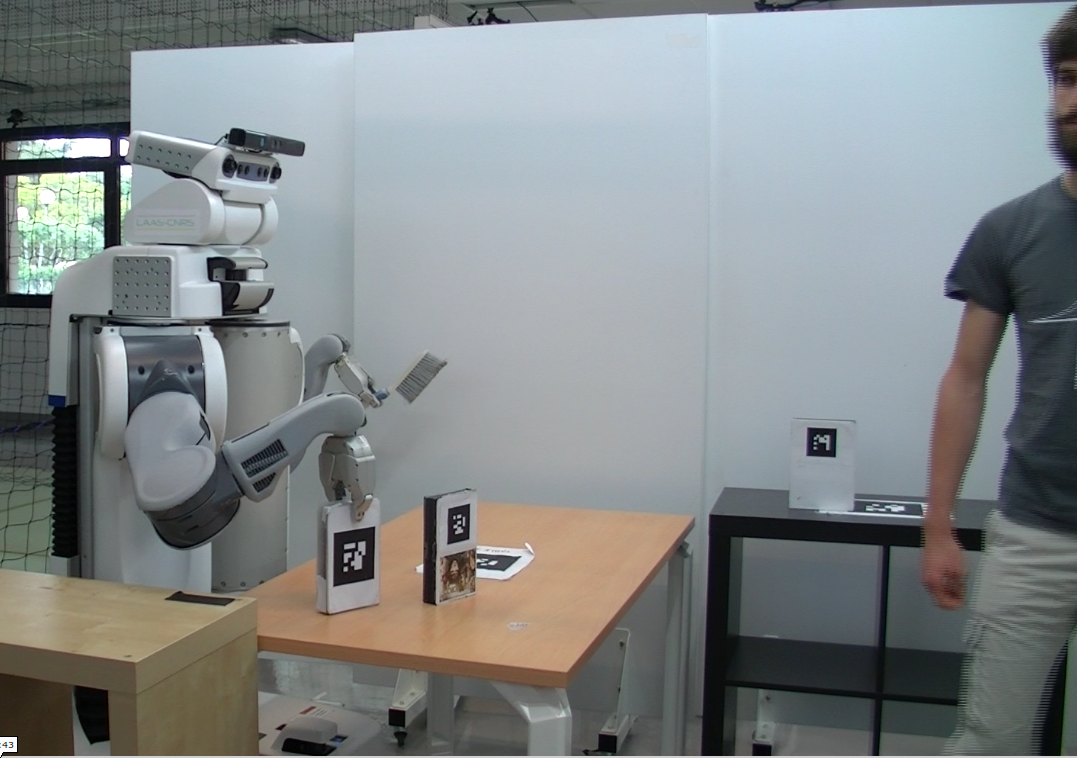
\includegraphics[width=0.4\textwidth]{figs/Chapter3/HumanLeave.png}
       \label{subfig:humanLeave}
   }
    %~
    \subfigure[The robot removes the last book and sweep the table.]{
        \centering
        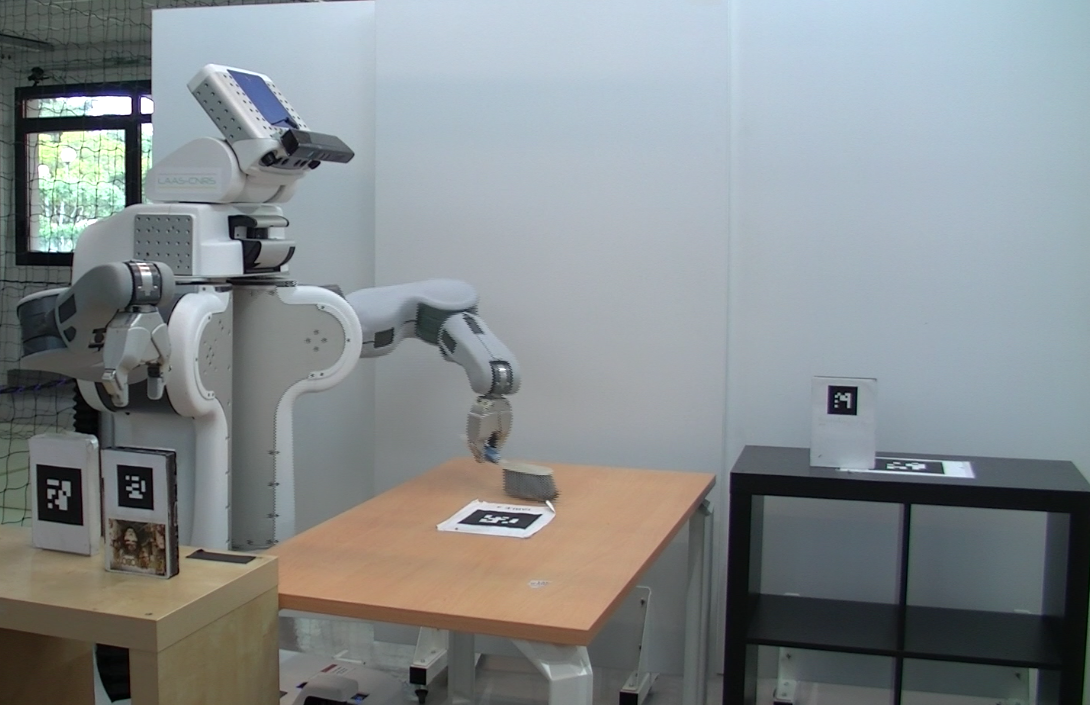
\includegraphics[width=0.44\textwidth]{figs/Chapter3/robotSweep.png}
       \label{subfig:robotSweep}
    }
    %~
    \subfigure[The human comes back.]{
        \centering
        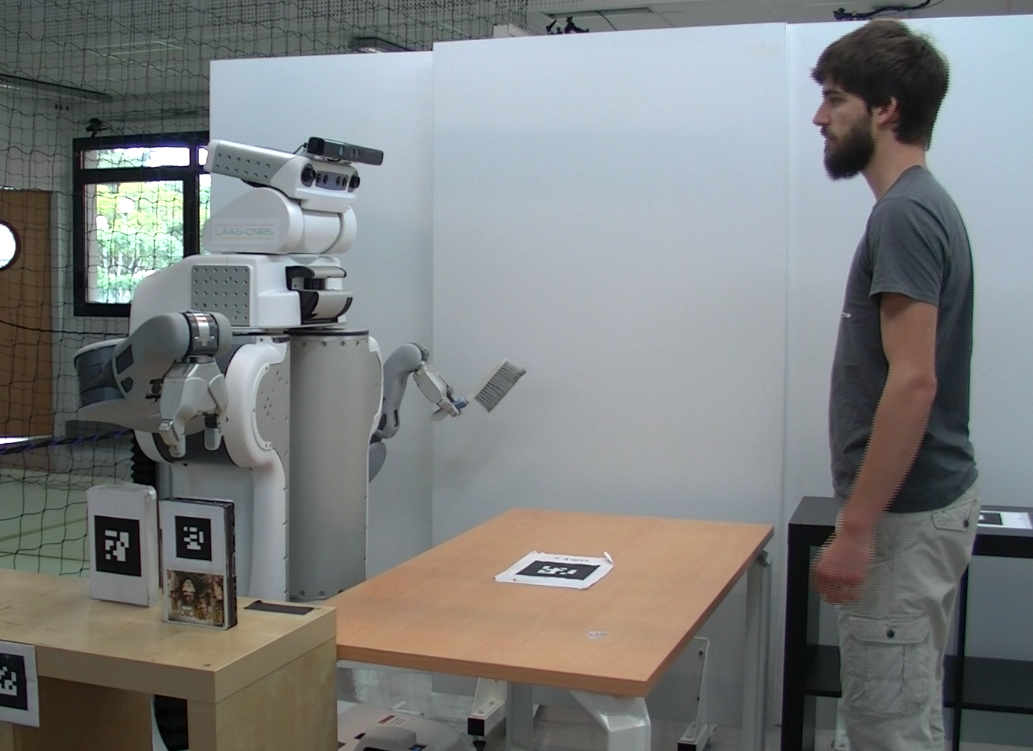
\includegraphics[width=0.4\textwidth]{figs/Chapter3/humanComesBack.png}
       \label{subfig:humanComesBack}
   }
    %~
    \subfigure[The human and the robot perform their last actions and achieve the task.]{
        \centering
        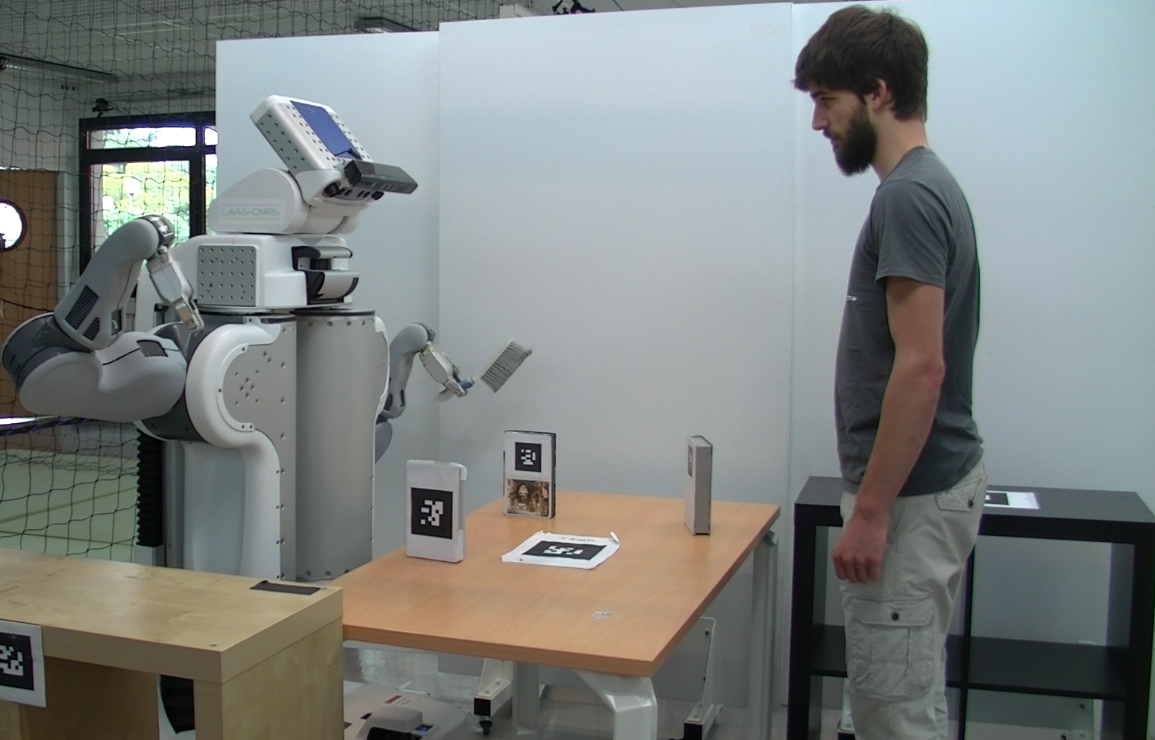
\includegraphics[width=0.45\textwidth]{figs/Chapter3/endClean.png}
       \label{subfig:endClean}
    }
    \caption{Illustrative "Clean the table" scenario.}
\end{figure*}

\subsection{Quantitative results}

We will now evaluate the benefits of the presented work in simulation in the two tasks described previously. Results in real situations as well as more simulation results with the whole system developed in the thesis can be found in Chapter~\ref{ch:Eval}). The results here only concern the use of mental states during Shared Plan execution.

When the interaction starts, we consider that the joint goal is already established and that a first Shared Plan has been computed by the robot. The robot executes the plan and the simulated human executes the actions planned for him. We randomly sample a time when the human leaves the scene and another time when the human comes back. While absent, the human does not execute actions and cannot see anything nor communicate.

One objective of our contribution is to reduce unnecessary communication from the robot during the execution of a Shared Plan aiming at a more friendly and less intrusive behaviour of the robot. Consequently, in order to evaluate our system, we have chosen to measure the amount of information shared by the robot during a Shared Plan execution. During the interaction, we logged the number of facts (information chunks) given by the robot to the human. An information concerns either a change in the environment or the state of a previous action. 

We compared our system (called \textit{ToM system}) to:
\begin{itemize}
\item a system which informs about each action missed by the human (called \textit{Missed system}).
\item a system informs about each action performed by the robot even if the human sees it (called \textit{Performed system}).
\end{itemize}

The obtained results in 100 runs are given in Table~\ref{table:results}.

\begin{table}[ht]
\begin{center}
\begin{tabular}{|r||c|c||c|c|}
\hline
 Scenario & \multicolumn{2}{c||}{Clean the table} & \multicolumn{2}{c|}{Inventory}\\
\cline{2-5} 
System & Average & Std Dev & Average & Std Dev\\
\hline
\hline
ToM & 0.94 & 0.24 & 0.41 & 0.48\\
\hline
Missed & 2.14 & 0.87 & 2.61 & 1.36\\
\hline
Performed & 3.72 & 0.96 & 10.0 & 0.0\\
\hline
\end{tabular}
\end{center}
\caption{Number of information given by the robot during the two presented scenarios for the three systems (\textit{TOM}, \textit{Missed} and \textit{Performed}).}
\label{table:results}
\end{table}

We can see that our system allows to reduce significantly the amount of information given by the robot. In the "Clean the table" scenario, depending on when the human leaves, the robot might change the initial plan and take care of the book reachable by both agents instead of the human. This explains why the average number for the \textit{Performed system} is higher than the number of actions initially planned for the robot: the robot performs more actions in the new plan. In this scenario, our system allows not to communicate about missed \textit{pickandplace} actions as the human can infer them by looking at the objects placements. However, the robot will inform the human if he missed the fact that the robot has swept the table as it is not observable and it is a necessary information for the human to know before he can put back objects on the table.

In the inventory scenario, as all objects and boxes are reachable only by one agent, the robot does not change the plan when the human leaves. This explains the fact that the standard deviation is null for the \textit{Performed system}: the number of actions performed by the robot never changes and there is no change in the plan. In this scenario, the \textit{pickanddrop} and \textit{scan} actions have non-observable effects (the human can not see an object in a box). However, we can see that our system still verbalizes less information than the \textit{Missed system}: the robot communicates only the information which the human really needs (as the fact that an object the human should drop in a box has been scanned) and does not give information which are not linked to the human part of the plan (as the fact that the robot scanned an object it have to drop in its box or that the robot dropped an object).


\section{Conclusion}

In this chapter we shown how we extended the robot estimation of humans mental states (which initially concerned only the environment) to the state of the task and more specifically of the Shared Plan. Then, we shown how we use these mental states to better communicate during Shared Plan execution.

The benefits of this work have been demonstrated with an illustrative example and simulation results. These results show that the proposed system allows to reduce communication by removing useless information given by the robot.

The next chapter will give more details about Shared Plan elaboration and management, more particularly concerning actions allocation. Then, we will show in Chapter~\ref{ch:Eval}) more complete simulation results with the whole system as well as results with the system running in a real situation.

\ifdefined\included
\else
\bibliographystyle{StyleThese}
\bibliography{These}
\end{document}
\fi
